%%%%%%%%%%%%%%%%%%%%%%%%%%%%%%%%%%%%%%%%%%%%%%%%%%%%%%%%%%%%%%%%
%%%%%%%%%%%%%%%%%%%%%%%%%%%%%%%%%%%%%%%%%%%%%%%%%%%%%%%%%%%%%%%%
%%%%
%%%% This text file is part of the source of 
%%%% `Introduction to High-Performance Scientific Computing'
%%%% by Victor Eijkhout, copyright 2012-2024
%%%%
%%%% This book is distributed under a Creative Commons Attribution 3.0
%%%% Unported (CC BY 3.0) license and made possible by funding from
%%%% The Saylor Foundation \url{http://www.saylor.org}.
%%%%
%%%%
%%%%%%%%%%%%%%%%%%%%%%%%%%%%%%%%%%%%%%%%%%%%%%%%%%%%%%%%%%%%%%%%
%%%%%%%%%%%%%%%%%%%%%%%%%%%%%%%%%%%%%%%%%%%%%%%%%%%%%%%%%%%%%%%%

%% for LaTeX newer than 2022-06-01:
%% \DocumentMetadata
%%     {
%%       testphase = phase-I
%%       }
\documentclass[11pt,fleqn,letterpaper,twoside,openany]{boek3}

%pyskipbegin
\input macros/comment.sty % use our own prerelease
\usepackage{verbatim}
\makeatletter
\def\verbatim@startline{\verbatim@line{\leavevmode\kern.5\unitindent\relax}}
\makeatother

\newif\ifIncludeAnswers
\IncludeAnswersfalse
\includecomment{tutorials}

\input inex

% fancy text stuff
\usepackage{fontspec}
\setmainfont[
  Extension=.otf,
  UprightFont={*-Regular},
  BoldFont={*-Bold},
  ItalicFont={*-Italic},
  BoldItalicFont={*-BoldItalic}
]{LibertinusSerif}
\usepackage{unicode-math}
\setmathfont{LibertinusMath-Regular.otf}

%% \usepackage{amssymb}
%% \usepackage[fleqn]{amsmath}


\usepackage[algo2e,noline,noend]{algorithm2e}
\newenvironment{displayalgorithm}
 {\par
  \begin{algorithm2e}[H]\leftskip=\unitindent \parskip=0pt\relax
  \DontPrintSemicolon
  \SetKwInOut{Input}{Input}\SetKwInOut{Output}{Output}
 }
 {\end{algorithm2e}\par}
\newenvironment{displayprocedure}[2]
 {\everymath{\strut}
  \begin{procedure}[H]\leftskip=\unitindent\caption{#1(#2)}}
 {\end{procedure}}

% for edmond
\usepackage{subfigure,algorithmic,algorithm}

\def\lulurevision{2016}

%
% page layout
%
\usepackage{geometry}
\addtolength{\textwidth}{.5in}
\addtolength{\textheight}{.5in}
\addtolength{\evensidemargin}{-.5in}

%%%%
%%%% Header handling
%%%%
\usepackage{fancyhdr}
\pagestyle{fancy}\fancyhead{}\fancyfoot{}
% remove uppercase from fancy defs
\makeatletter
\def\chaptermark#1{\markboth {{\ifnum \c@secnumdepth>\m@ne
 \thechapter. \ \fi #1}}{}}
\def\sectionmark#1{\markright{{\ifnum \c@secnumdepth >\z@
 \thesection. \ \fi #1}}}
\makeatother
% now the fancy specs
%\fancyhead[LE]{\thepage \hskip.5\unitindent/\hskip.5\unitindent \leftmark}
%\fancyhead[RO]{\rightmark \hskip.5\unitindent/\hskip.5\unitindent \thepage}
\fancyhead[LE]{\leftmark}
\fancyfoot[LE]{\thepage}
\fancyhead[RO]{\rightmark}
\fancyfoot[RO]{\thepage}
\fancyfoot[RE]{\footnotesize\sl Introduction to High Performance
  Scientific Computing}
\fancyfoot[LO]{\footnotesize\sl Victor Eijkhout}

\setlength{\headheight}{14pt}
\addtolength{\topmargin}{-2pt}

\input exmacs

\newwrite\nx
\newcommand\CHAPTER[2]{
\Level 0 {#1}\label{ch:#2}
\def\chapshortname{#2}
{\SetBaseLevel 1 \input chapters/#2
 \write\chapterlist{\chapshortname}
 \openout\nx=exercises/\chapshortname-nx.tex
 \write\nx{\arabic{excounter}}
 \closeout\nx
 \SetBaseLevel 0
}}

\newcommand\APPLICATION[2]{
\Level 0 {#1}\label{app:#2}
\def\chapshortname{#2}
{\SetBaseLevel 1 \input applications/#2
 \write\chapterlist{\chapshortname}
 \openout\nx=exercises/\chapshortname-nx.tex
 \write\nx{\arabic{excounter}}
 \closeout\nx
 \SetBaseLevel 0
}}

\newcommand\TUTORIAL[2]{
\vfill\pagebreak \Level 0 {#1}\label{tut:#2}
\def\chapshortname{#2}\setcounter{excounter}0\relax
{\SetBaseLevel 1 \input tutorials/#2
\write\chapterlist{\chapshortname}
\openout\nx=exercises/\chapshortname-nx.tex
\write\nx{\arabic{excounter}}
\closeout\nx
\SetBaseLevel 0
}}
\newif\ifprojects\projectsfalse
\newcommand\PROJECT[2]{
\ifprojects \vfill\pagebreak \else \projectstrue \fi
\Level 1 {#1}\label{prj:#2}
\def\chapshortname{#2}
{\SetBaseLevel 2 \input projects/#2
\write\chapterlist{\chapshortname}
\openout\nx=exercises/\chapshortname-nx.tex
\write\nx{\arabic{excounter}}
\closeout\nx
\SetBaseLevel 0
}}
\newcommand\APPENDIX[2]{
  \vfill\pagebreak \Level 0 {#1}\label{app:#2}
  \def\chapshortname{#2}
  {\SetBaseLevel 1 %% {\index{#2|(textbf}}
   \setcounter{excounter}0
   \input appendices/#2 %%{\index{#2|)}}
   \write\chapterlist{\chapshortname}
   \openout\nx=exercises/\chapshortname-nx.tex
   \write\nx{\arabic{excounter}}
   \closeout\nx
   \SetBaseLevel 0
  }
}

\newcommand\maillink[3]{
  \href{mailto:eijkhout@tacc.utexas.edu?subject=comment on section #1 "#2"}
    {comments on this #3?}\par
}
\renewcommand\maillink[3]{}

\newif\ifInBook \InBooktrue
\input scimacs
\input acromacs
\input blockmacs
\input bookmacs
\externaldocument[CARP-]{scicomptutorials}
\input listingmacs
\def\codesnippetsdir{snippets.code}
\def\tutsnippetsdir{snippets}
\input snippetmacs
\input tutmacs
\input idxmacs
\input tikzplot

\begin{notlulu}
  \usepackage[xetex,colorlinks,pagebackref=true]{hyperref}
  \hypersetup{bookmarksopen=true}
  \renewcommand*{\backref}[1]{}
  \renewcommand*{\backrefalt}[4]{[{\tiny%
      \ifcase #1 Not cited.%
      \or Cited on page~#2.%
      \else Cited on pages #2.%
      \fi%
  }]}
  \usepackage[all]{hypcap}
\end{notlulu}
\begin{lulu}
  \usepackage{url}
\end{lulu}

\makeindex

%\tracingmacros=2
%\tracingcommands=2

\def\publicdraft{{\bf\normalsize \\Evolving Copy - open for comments}}
\def\revdate{3rd edition 2022, formatted \today\\
  Series reference: \url{https://theartofhpc.com}\\
  This book is published under the CC-BY 4.0 license.
}
\begin{lulu}
  \def\publicdraft{}
  \def\revdate{3rd edition 2022\\
    Series reference: \url{https://theartofhpc.com}\\
    This book is published under the CC-BY 4.0 license.
  }
\end{lulu}

\author{Victor Eijkhout\\ with\\Edmond Chow, Robert van de Geijn}
\title{The Science of Computing
  \\
    {\small The Art of High Performance Computing, volume 1}
    \\
    \publicdraft
}
\expandafter\date\expandafter{\revdate}

\newwrite\chapterlist \openout\chapterlist=chapternames.tex

\begin{document}
%\dosecttoc
\maketitle

\input copyright
\input introduction

\vfill\pagebreak 
{\setcounter{tocdepth}{1}
\tableofcontents
\setcounter{tocdepth}{2}
}

%pyskipend

\part{Theory}

\CHAPTER{Single-processor Computing}{sequential}
\CHAPTER{Parallel Computing}{parallel}
\CHAPTER{Computer Arithmetic}{arithmetic}
\CHAPTER{Numerical treatment of differential equations}{odepde}
\CHAPTER{Numerical linear algebra}{linear}
\CHAPTER{Programming for performance}{performance}
\CHAPTER{High performance linear algebra}{parallellinear}

\part{Applications}

\APPLICATION{Molecular dynamics}{md}

\begin{lulu}
  \APPLICATION{Sorting}{sorting}
\end{lulu}
\begin{notlulu}
  \APPLICATION{Combinatorial algorithms}{combinatorics}
\end{notlulu}

\APPLICATION{Graph analytics}{graphalgorithms}
\APPLICATION{N-body problems}{discrete}

\begin{montecarlo}
\APPLICATION{Monte Carlo Methods}{montecarlo}
\end{montecarlo}

\APPLICATION{Machine learning}{learning}

\begin{notready}
\APPLICATION{Computational biology}{bio}
\APPLICATION{Big data}{analytics}
\APPLICATION{Computer graphics}{graphics}
\APPLICATION{Quantum computing}{quantum}
\end{notready}

% not for public consumption
\begin{notready}
%% https://scicomp.stackexchange.com/questions/42997/lattice-boltzmann-method-parallelization/43011#43011
\APPLICATION{Other physics applications}{lbm}
\end{notready}

\begin{comment}
%%\CHAPTER{Performance measurement and optimization}{performance}
%%\CHAPTER{Applications}{applications}
%%\CHAPTER{Scientific Programming}{programming}
\end{comment}

\part{Appendices}
\setcounter{tocdepth}{2}

%\Level 0 {Theoretical background}

\input appendices/blurb

% arg 2 is term in the index
\APPENDIX{Linear algebra}{norms}
\APPENDIX{Complexity}{complexity}
\APPENDIX{Partial Differential Equations}{pde}
\APPENDIX{Taylor series}{taylor}
\APPENDIX{Minimization}{newton}
\APPENDIX{Random numbers}{random}
\APPENDIX{Graph theory}{graph}
\begin{notready}
\APPENDIX{Fourier Transforms}{fft}
\end{notready}
\APPENDIX{Automata theory}{fsa}
\APPENDIX{Parallel Prefix}{prefix}

%pyskipbegin

\part{Projects, codes}

\Level 0 {Class projects}

Here are some suggestions for end-of-semester projects
that feature a combination of coding and analysis.

\CHAPTER{Teaching guide}{teaching}
\PROJECT{Cache simulation and analysis}{cache}
\PROJECT{Evaluation of Bulk Synchronous Programming}{bsp}
\PROJECT{Heat equation}{heat}
\PROJECT{The memory wall}{wall}

\Level 0 {Codes}
\label{app:codes}
\input appendices/codes

\part{Indices}

\Level 0 {Index}

\addcontentsline{toc}{chapter}{Index of concepts and names}
\index{cluster!node|see{node}}
\index{CPU-bound|see{compute-bound}}
\index{directives|see{compiler, directives}}
\index{GNU!gdb|see{gdb}}
\index{halo|see{ghost region}}
\index{irreducible|see{reducible}}
\index{modified Gramm-Schmidt|see{Gram-Schmidt, modified}}
\index{parallel prefix|see{prefix operation}}
\index{Roadrunner|see{IBM!Roadrunner}}

\begin{multicols}{2}
  \printindex
\end{multicols}

\Level 0 {List of acronyms}

\begin{multicols}{2}
\begin{description}
\input acronyms
\end{description}
\end{multicols}
%\vfill\pagebreak

\Level 0 {Bibliography}

\bibliography{vle}
\bibliographystyle{plain}

%%%%%%%%%%%%%%%%
%%%% close business
%%%%%%%%%%%%%%%%

\hbox{}\vfill
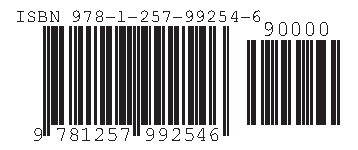
\includegraphics{isbn_barcode}

\closeout\chapterlist

%pyskipend
\end{document}
